%----------------------------------------------------------------------------
\chapter{Background}
%----------------------------------------------------------------------------
%TODO review LTS "path" and "trace" everywhere
TODO 

\section{Model-Based Engineering}
Due to the application of the modeling concept in several completely different domains, first of all, we need to define the meaning of \textit{model}.
\begin{definition}[Model]
	A model is the simplified image of an element of the real or a hypothetical world (the system), that replaces the the system in certain considerations.
\end{definition}

For a model to be interpretable, executable or formally verifiable, it must be described according to predefined rules in the given domain. This set of rules is provided by \textit{modeling languages}.
\begin{definition}[Modeling Language]
	A modeling language consists of the following elements:
	\begin{itemize}
		\item \emph{Metamodel:} a model defining the building blocks of the modeling language as well
		as their relationships.
		\item \emph{Concrete syntax:} a set of rules defining a graphical or textual notation for the
		element and connection types defined in the metamodel.
		\item \emph{Well-formedness constraints:} a set of constraints that models have to meet in order
		to be deemed valid in the modeling language.
		\item \emph{Semantics:} a set of rules that define the meaning of the element and connection
		types defined in the metamodel. Semantics can be either \textit{operational} (what should happen during execution) or \textit{denotational} (given by translating concepts in a modeling language to another modeling language with well-defined semantics).
	\end{itemize}
\end{definition}

Models can grasp various aspects of a system. Structural models describe the structure of the system, representing knowledge regarding the parts of the system and the properties and connections of these parts. This means that the model describes static knowledge and not temporal change. On the other hand, behavioral models describe the change of the system over time through its changing of states and execution of processes. These categories do not cover every aspect of a system, and usually cannot be separated this well in practical applications. For instance, action languages of state-based models describe the behavior of the system in a procedural way. There are several possible formalisms for both kinds of models, some of which are discussed in Section %TODO%\ref{sec_backgrmodeling}.

The process of deriving design artifacts is called \textit{model transformation}.
\begin{definition}[Model Transformation]
	Model transformation is the process of generating the target model from the source model. This process is described by by a transformation definition consisting of transformation rules, and a transformation tool that executes them. A transformation rule is the mapping of elements of the source model to the elements of the target model. \cite{ModelTransformation}
\end{definition}

Model transformations can be categorized based on the types of the source and target models: model-to-model (M2M), model-to-text (M2T), text-to-model (T2M) and text-to-text (T2T). These categories fundamentally define the tools required and usable for handling the different models.

There are also two important factors to consider when designing a model transformation: 
\begin{itemize}
	\item \textit{Consistency}: the same structure or behavior is described by the source and the target models (in their respective domains).
	\item \textit{Traceability}: the images of the original elements of the source model can be traced back to the original elements, from which they were generated.
\end{itemize}

\textbf{Model-Based Systems Engineering (MBSE)} is the formalized application of modeling to support system requirements, design, analysis, verification and validation activities beginning in the conceptual design phase and continuing throughout development and later life cycle phases\cite{mbse}. This concept can also be applied to software engineering. Note, that the models may be the primary artifact of the development process, in which case precisely defined formal models are required. When the models are the primary artifacts, the process is called \textit{Model-Driven Engineering}.


\section{Foundations of Automata Theory}
In order to provide the theoretical background of behavioral modeling, this section discusses the necessary basics of formal language and automata theory.

First, we introduce the fundamentals of formal language theory, on which automaton theory is based. 

\subsection{Fundamentals of Formal Language Theory}
Atomic elements of formal languages are alphabets, characters and words.

\begin{definition}[Alphabet]
	Let $\Sigma$ be a finite, non-empty set. $\Sigma$ is an alphabet, its elements are symbols or characters.
\end{definition}

\begin{definition}[Word]
	If $\Sigma$ is an alphabet, then any finite sequence comprised of the symbols of $\Sigma$ are words (or Strings). $\Sigma^{n}$ represents the set of every $n$ length word consisting of symbols in $\Sigma$: $\Sigma^{n}: w_1w_2\ldots w_n$, where $\forall 0 \leq i \leq n: w_i \in \Sigma$. The set of every finite word under an alphabet, formally $\bigcup\limits_{n>0}^{} \Sigma^{n}$ is denoted by $\Sigma^{*}$. The empty word is denoted by $\epsilon$. Any word $w$ with a length $n$ can be viewed as a function $w: \{0, 1, ..., n-1\} \rightarrow \Sigma$.
\end{definition}

Words can be constructed using other words. The following definition defines these relations.

\begin{definition}[Prefixes, Substrings and Suffixes]
	Let an arbitrary $w = uvs$, where $w, u, v, s\in\Sigma^*$. $u$ is the prefix, $v$ is the substring, and $s$ is the suffix of $w$. Formally:
	\begin{itemize}
		\item $w\in\Sigma^*$ is a prefix of $u\in\Sigma^*$ iff $\exists s\in\Sigma^*: s=wu$,
		\item $w\in\Sigma^*$ is a suffix of $u\in\Sigma^*$ iff $\exists s\in\Sigma^*: s=uw$,
		\item $w\in\Sigma^*$ is a substring of $u, v\in\Sigma^*$ iff $u$ is the prefix and $v$ is the suffix of $w$.
	\end{itemize}
\end{definition}

Using these atomic elements of formal language theory, formal languages can be defined.

\begin{definition}[Formal Language]
	An arbitrary set of words under an Alphabet $\Sigma$ is a Language. Formally: $L\subseteq\Sigma^{*}$.
\end{definition}

\begin{definition}[Prefix-closure]
	Let $L\subseteq\Sigma^*$ and $L' = \{u\in\Sigma^*, v\in\Sigma^* : uv\in L\}$. In other words, L' is the set containing all the prefixes of every word of L. L is prefix-closed if $L = L'$.
\end{definition}

Especially in case of describing the behavior of reactive systems (or non-terminating programs), it makes sense to introduce the infinitary counterparts of these definitions. In the following, we use $\omega$ to denote the first infinite ordinal -- as it is customary in set theory. %TODO ref (e.g. learnability of infinitary regular sets)

\begin{definition}[$\omega$-Sequence]
	If $\Sigma$ is an alphabet, then any infinite sequence comprised of the symbols of $\Sigma$ are $\omega$-sequences (also called infinite sequences or infinite words). Any $\omega$-sequence $\alpha$ can be viewed as a function $\alpha: \mathbb{N} \rightarrow \Sigma$. The set of all $\omega$-sequences is denoted $\Sigma^\omega$.
\end{definition}

%TODO is this needed?
\begin{definition}[Ultimately Periodic Word]
	Every $\alpha \in \Sigma ^ \omega$ has infinitely many factorizations of the form $\alpha = u \beta$ into a finite prefix $u$ and an infinite suffix $\beta$. Given a finite sequence $u, u^\omega$ is the infinite sequence obtained by concatenating infinitely many instances of $u$. An infinite sequence $\alpha$ that admits a factorization of the form $uv^\omega$ is said to be $ultimately$ $periodic$.
\end{definition}

\begin{definition}[$\omega$-Language]
	An arbitrary set of infinite words under an Alphabet $\Sigma$ is an $\omega$-Language. Formally: $L\subseteq\Sigma^\omega$.
\end{definition}


Formal language theory is closely linked with automata theory, which we will introduce in the following subsection.

\subsection{Finite Automata and $\omega$-automata} \label{ss:automata}

Informally, automata are mathematical constructs which read characters from an input and classify them into "accepted" and "rejected" categories. A bit more precisely, automata consist of states, some of which are accepting states. Starting from an initial state, based on the inputs received, the automaton transitions between states. If after processing a sequence of inputs, the final state of the automaton is an accepting state, the input sequence is accepted. If not, the input is rejected.

One of the simplest automata is the Deterministic Finite Automaton.

\begin{definition}[Finite Automaton]
	A Finite Automaton is a Tuple of $ DFA=(S,s_{0},\Sigma,\delta,F) $, where: 
	\begin{itemize}
		\item S is a finite, non-epty set containing the states of the automaton,
		\item $s_{0} \in S$ is the initial state,
		\item $\Sigma$ is a finite Alphabet,
		\item $\delta: S\times \Sigma \to S$ is a transition function,
		\item $F\subseteq S$ is a set of the accepting states of the automaton. 
	\end{itemize}
\end{definition}

One kind of finite automata, called $Deterministic$ $Finite$ $Automata$ $(DFA)$ refer to a property of every state having exactly one transition for every input. Formally: $\delta (s,a) \in S$, where $s \in S$ and $a \in \Sigma \cup \{\epsilon\}$ .

The other kind of finite automata, called $Nondeterministic$ $Finite$ $Automata$ $(NFA)$ refer to a property of every state possibly having multiple transitions or maybe none for any given input. Formally: $\delta (s,a) \in S$, where $s \subseteq S$ and $a \in \Sigma$ .

An example of a DFA (Deterministic Finite Automaton) from\cite{Steffen2011} can be seen in Example \ref{ex:dfaexample}.

\begin{example}
	\label{ex:dfaexample}
	See Figure \ref{fig:dfaexample}. This example has four states, $S = \{q_0, q_1, q_2, q_3\}$ (hence $|S| = 4$). The initial state is marked by the start arrow, so $s_0 = q_0$. The alphabet can be inferred as $\Sigma = \{a, b\}$. Transitions are visualized as $q_0$ $\xrightarrow[]{\text{a}}$ $q_1$ given by the transition function (in this example) $\delta(q_0, a) = q_1$. The complete transition function in a table form can be seen in Table \ref{tab:dfaexampledelta}. Finally, the accepting states, or in this case, accepting state of the automaton is $F = \{q_3\}$.
\end{example}


The semantics of automata are defined via runs. A run of an automaton is to test for a certain input (word), if it is accepted or rejected. See Example \ref{ex:dfaruns}.

\begin{example}
	\label{ex:dfaruns}
	In accordance with the transition function, a run of Figure \ref{fig:dfaexample} with an input of $\{a, a, a\}$ would end in state $q_3$ meaning the input is accepted. A rejected input could be $\{a, b, b\}$, which would stop at state $q_1$, a non-accepting state. On deeper examination, one can see, that this automaton only accepts runs with inputs containing $4i+3 a$.
\end{example}

\begin{figure}[!ht]
	\centering
	\begin{tikzpicture}[shorten >=1pt,node distance=3cm,on grid,auto] 
		\node[state,initial] (q_0)   {$q_0$}; 
		\node[state] (q_1) [right=of q_0] {$q_1$}; 
		\node[state] (q_2) [below=of q_0] {$q_2$}; 
		\node[state,accepting](q_3) [right=of q_2] {$q_3$};
		\path[->] 
		(q_0) edge  node {a} (q_1)
		edge [loop below] node {b} ()
		(q_1) edge  node[pos=0.62]  {a} (q_2)
		edge [loop below] node {b} ()
		(q_2) edge  node [swap] {a} (q_3) 
		edge [loop above] node {b} ()
		(q_3) edge  node[pos=0.62] [swap] {a} (q_0)
		edge [loop above] node {b} () ;
	\end{tikzpicture}
	\caption{A simple DFA from \cite{10.1007/978-3-319-11164-3_26}.}
	\label{fig:dfaexample}
\end{figure}

\begin{table}[!ht]
	\centering
	\begin{tabular}{|c|cccc|}
		\hline
		$\delta$ & $q_0$ & $q_1$ & $q_2$ & $q_3$\\ \cline{1-5}
		a & $q_1$ & $q_2$ & $q_3$ & $q_0$ \\	
		b & $q_0$ & $q_1$ & $q_2$ & $q_3$ \\	\hline
	\end{tabular}
	\caption{The transition function of the automaton seen in Figure \ref{fig:dfaexample}}
	\label{tab:dfaexampledelta}
\end{table}


A slightly different formalism can be defined for cases where the acceptance of the input (word) is not necessary to consider, called Labeled Transition System.

\begin{definition}[Labeled Transition System]
	A Labeled Transition System is a Tuple $LTS=(S, Act, \rightarrow)$, where:
	\begin{itemize}
		\item $S={q_0, q_1, ..., q_n}$ the finite, non-empty set of states, $q_0$ being the initial state,
		\item $Act = {a, b, c, ...}$ the finite set of actions,
		\item $\rightarrow \subseteq S \times Act \times S$ the labeled transitions between the states.
	\end{itemize}
	In the beginning, the initial state is active. The active state may change after each transition.
	
	The \textit{path} of an LTS is the $\pi = (q_0, a_1, q_1, a_2, ...)$ alternating sequence of states and actions, where $q_0$ is the initial state and the subsequent states are the results of the transitions labeled with the actions of the same index, starting from the state with the previous index. 
\end{definition}

\begin{example}
	\label{ex:ltsexample}
	See Figure \ref{fig:ltsexample}. This example has three states, $S = \{q_0, q_1, q_2\}$ (hence $|S| = 3$). The initial state is $q_0$, also marked by the start arrow. The set of actions is $Act = \{money, coffee, tea\}$. Transitions are visualized as $q_0$ $\xrightarrow[]{\text{money}}$ $q_1$ given by the transition (in this example) $(q_0, money, q_1)$. The set of transitions ($\rightarrow$) also contains $(q_1, coffee, q_2)$ and $(q_1, tea, q_3)$.
\end{example}

\begin{figure}[!ht]
	\centering
	\begin{tikzpicture}[shorten >=1pt,node distance=3cm,on grid,auto] 
		\node[state, initial] (s_1)   {$q_0$}; 
		\node[state] (s_2) [below=of s_1] {$q_1$}; 
		\node[state] (s_3) [left=of s_2] {$q_2$}; 
		\node[state](s_4) [right=of s_2] {$q_3$};
		\path[->] 
		(s_1) edge  node {money} (s_2)
		(s_2) edge  node[pos=0.62]  {coffee} (s_3)
		(s_2) edge  node [swap] {tea} (s_4) ;
	\end{tikzpicture}
	\caption{A simple LTS}
	\label{fig:ltsexample}
\end{figure}

Finite automata and LTSs are useful to model system behavior based on inputs, but in order to work with reactive systems, we also need to handle outputs. Mealy machines are (usually deterministic) automata designed to communicate with output symbols instead of accepting and rejecting states.


\begin{definition}[Mealy Machine]
	A Mealy machine or Mealy automaton is a Tuple of $ M=(S,s_{0},\Sigma,\Omega,\delta,\lambda) $, where:
	\begin{itemize}
		\item S is a finite, non-empty set containing the states of the automaton,
		\item $s_{0} \in S$ is the initial state,
		\item $\Sigma$ is the input alphabet of the automaton,
		\item $\Omega$ is the output alphabet of the automaton,
		\item $\delta: Q\times \Sigma \to Q$ is the transition function and
		\item $\lambda: Q\times \Sigma \to \Omega$ is the output function. 
	\end{itemize}
\end{definition}

Mealy machines can be regarded as deterministic finite automata over the union of the input alphabet and an output alphabet with just one rejection state, which is a sink, or more elegantly, with a partially defined transition relation.\cite{Steffen2011}

An example of a deterministic Mealy machine can be seen in Example \ref{ex:coffeemealy}.

\begin{example}
	\label{ex:coffeemealy}
	An example of a deterministic Mealy machine can be seen in Figure \ref{fig:coffeemealy}. The formal definition of the automaton can be seen below.
	\begin{itemize} 
		\item $S = \{a, b, c, d, d', e, f\}$ 
		\item $s_0 = a$
		\item $\Sigma = \{water, pod, button, clean\}$
		\item $\Omega$ = \{$\checkmark$, \Coffeecup, $\star$\}
	\end{itemize}
	The transitions, as seen in Figure \ref{fig:coffeemealy} are visualized as $s_0$ $\xrightarrow[]{\text{input/output}}$ $s_1$, which denotes the machine moving from state $s_0$ to state $s_1$ on the specified input, while causing the specified output. Also, some simplifications are done, e.g. in this transition: d $\xrightarrow[]{\text{\{water,pod\}/\checkmark}}$ d we see a visual simplification of having both transitions merged to one arrow, this is only for visual convenience. Figure \ref{fig:coffeemealy} is also a great example of sinks, as seen in state f, the machine accepts anything, and never changes. This is a variation of the accepting state seen in DFAs.
\end{example}

\begin{figure}[!ht]
	\centering
	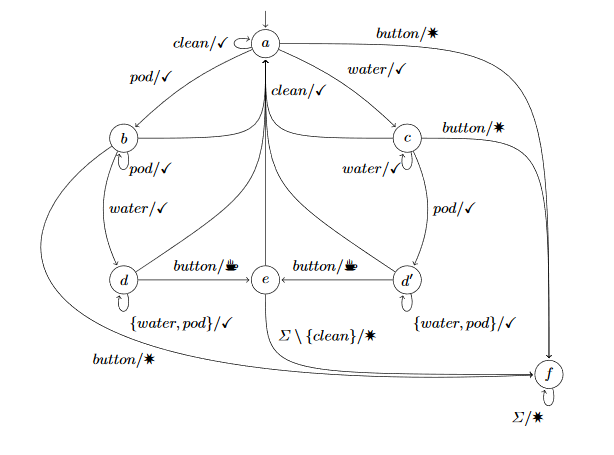
\includegraphics[width=0.7\linewidth]{figures/coffeemealy}
	\caption{Mealy machine representing the functionality of a coffee machine.\cite{Steffen2011}}
	\label{fig:coffeemealy}
\end{figure}

Another possible extension of finite automata is the acceptance of infinite input sequences. These automata are called $\omega$-$automata$, most of which are nondeterministic and differ only in their acceptance condition. The most notable kinds of $\omega$-automata are Büchi, Co-Büchi, Rabin, Streett, parity and Muller automata, some of which are defined here. 

%TODO other ref, this one is only for Büchi
%TODO transition-based definition: only that is important later
\begin{definition}[$\omega$-Automaton \cite{majzikform}]
	An $\omega$-automaton is a tuple $A=(S, s_0, \Sigma, \delta, F)$, where:
	\begin{itemize}
		\item $S=\{0,1, ..., k\}$ for some $k \in \mathbb{N}$. A finite, non-empty set containing the states of the automaton, 
		\item $s_0 \subseteq S$ is the set of initial states,
		\item $\Sigma$ is a finite alphabet,
		\item $\rho : S \times \Sigma \rightarrow 2^S$ is the nondeterministic transition function,
		\item $F \subseteq S$ is a set of the final states of the automaton.
	\end{itemize}
	
	A run of the $\omega$-automaton $A$ is the $r=(s_0,s_1,s_2,...)$ infinite series of states as a result of an $a_0, a_1, a_2, ...$ infinite input (word), where $s_0 \in S_0$ and $\forall s_{i+1}=\rho(s_i, a_i)$. 
	
	The characteristic of an infinite run is the set of $s \in S$ states, which occur infinitely many times during the run. Formally: $lim(r) = \{s | \nexists j \geq 0 : \forall k > j : s \neq s_k\}$. 
	
	\textbf{Büchi Acceptance Condition:} A run of the Büchi-automaton is accepting, if $lim(r) \cap F \neq \emptyset$. A $ w $ infinite word is accepted by the automaton, if there exists a run of the automaton that accepts $w$.
	
	\textbf{Co-Büchi Acceptance Condition:} A run of the Co-Büchi-automaton is accepting, if $lim(r) \subseteq F$. A $ w $ infinite word is accepted by the automaton, if there exists a run of the automaton that accepts $w$.
	
	\textbf{Parity Acceptance Condition:} A run of the parity automaton is accepting, if $min(lim(r))$ is even. A $ w $ infinite word is accepted by the automaton, if there exists a run of the automaton that accepts $w$.
\end{definition}

\begin{example}
	\label{ex:buchiexample}
	Figure \ref{fig:buchiexample} shows a simple Büchi automaton. Notice the nondeterminism and how the automaton accepts only infinite runs. 
\end{example}

\begin{figure}[!ht]
	\centering
	\begin{tikzpicture}[shorten >=1pt,node distance=3cm,on grid,auto] 
		\node[state, initial] (q_0)   {$q_0$}; 
		\node[state] (q_1) [right=of q_0] {$q_1$}; 
		\node[state, accepting] (q_2) [right=of q_1] {$q_2$}; 
		\node[state, accepting](q_3) [below=of q_0] {$q_3$};
		\path[->]
		(q_0) edge node {$true$} (q_1)
		(q_1) edge node {$\neg a$} (q_2)
		(q_0) edge [bend left=60] node {$\neg a$} (q_2)
		(q_0) edge [bend left=60] node {$b$} (q_3)
		(q_0) edge [bend right=60] node {$\neg b$} (q_3)
		(q_1) edge [loop below] node {$true$} ()
		(q_2) edge [loop below] node {$\neg a$} ()
		(q_3) edge [loop right] node {$b$} ()
		(q_3) edge [loop left] node {$ \neg b$} ();
	\end{tikzpicture}
	\caption{A simple Büchi-automaton}
	\label{fig:buchiexample}
\end{figure}

%TODO more examples: co-büchi, parity automata (maybe for the same GFa->GFb)

%TODO hierarchy of omega automata or theorem for equivalence of expressive power

Since automaton-based formalisms deal with alphabets, formal language theory is essential not only to define them, but to construct them in a way that is efficient in practical applications. Often automata are used to design and analyze real-life systems. Naturally, questions of efficiency and correctness arise, which is why the relations of automata and formal languages are discussed more in-depth in the following subsection.

\subsection{Relations of Formal Languages and Automata}
\begin{definition}[Recognized language of automata]
	The language $L\subseteq\Sigma$ containing all the accepted words by an automaton M is called the recognized language of the automaton. It is denoted by L(M) = L.
\end{definition}

\begin{definition}[Regular language]
	A formal language L is regular, iff there is a Deterministic Finite Automaton M, for which L(M) = L, in other words, iff there is a DFA with the recognized language of L.
\end{definition}

Let us now introduce a semantic helper $\delta^*$ for both DFAs and Mealy machines. $\delta^*$ is an extension of the $\delta$ transition function, as $\delta^*: S\times\Sigma^* \to S$ defined by $\delta^*(s,\epsilon) = s$ and $\delta^*(s, \alpha w) = \delta^*(\delta(s, \alpha), w)$, essentially providing the state of the automaton after running an input sequence from a specified state.

\begin{definition}[Myhill-Nerode relation] 
	A DFA $M=(S,s_{0},\Sigma,\delta,F)$ induces the following equivalence relation $\equiv_M$ on $\Sigma^*$ (when L(M) = $\Sigma$):\\
	\null\qquad$x\equiv_M y \iff \delta^*(s, x) = \delta^*(s, y)$\\
	where $x, y\in\Sigma^*$. This means, that x and y are equivalent with respect to $\equiv_M$.\cite{Kozen1977}.
\end{definition}

In words, the Myhill-Nerode relation states, that two words are equivalent wrt. $\equiv_M$ iff runs of both words would end in the same state on the automaton M. The Myhill-Nerode relation is an equivalence relation with some additional properties\cite{Kozen1977}, which can be seen in the following.


\begin{itemize}
	\item The properties of equivalence relations:
	\begin{itemize}
		\item Reflexivity: $x\equiv_M x$.
		\item Symmetry: $x\equiv_M y \implies y\equiv_M x$.
		\item Transitivity: if $(x\equiv_M y$ and $y\equiv_M z) \implies x\equiv_M z$.
	\end{itemize}
	\item Right congruence: $\forall x, y\in\Sigma^*: (x\equiv_M y \implies 		\forall a\in\Sigma: xa\equiv_Mya)$\\ also, by induction, this can be extended to:\\
	$\forall x, y\in\Sigma^*: (x\equiv_M y \implies \forall w\in\Sigma^*: xw\equiv_Myw)$. 
	\item It respects membership wrt. R:\\
	$\forall x, y\in\Sigma^*: x\equiv_M y \implies (x\in R \iff y\in R)$.
	\item $\equiv_M$ is of finite index, has finitely many equivalency classes. Since for every state $s\in S$, the sequences which end up in s are in the same equivalence class, the number of these classes is exactly $|S|$, which is a finite set.
\end{itemize}

Using this relation, we can introduce the Myhill-Nerode theorem, which neatly ties together the previous definitions.

\begin{theorem}[Myhill-Nerode theorem\cite{Kozen1977}\cite{10.2307/2033204}]\label{theorem:Myhill-Nerode}
	Let $L\subseteq\Sigma^*$. The following three statements are equivalent:
	\begin{itemize}
		\item L is regular.
		\item there exists a Myhill-Nerode relation for L.
		\item the relation $\equiv_L$ is of finite index.
	\end{itemize}
	For proof, see \cite{Kozen1977}\cite{10.2307/2033204}.
\end{theorem}

The same concepts can be applied to Mealy machines, which are somewhat more complex in this regard. As before, a semantic helper is needed similar to $\delta^*$, but considering the output function of Mealy machines. $\lambda^*: S\times\Sigma^* \to \Omega$, defined by $\lambda^*(s, \epsilon) = \varnothing$ and $\lambda^*(s, w\alpha) = \lambda(\delta^*(s, w), \alpha)$.



When monitoring the behavior of Mealy machines, one of the most important metrics given an input is the specific output given by the input. The behavior of a Mealy machine, a specific run of it, has a pattern of \textit{$i_1,o_1,i_2,o_2,..,i_n,o_n$}, where \textit{i} are inputs and \textit{o} are outputs. In order to characterize these runs, we actually do not need every output from this pattern, we only need the final one. Also note, that essentially the final output of a run is given by $\lambda^*(s_0, inputs)$. Let us introduce a $\llbracket M\rrbracket$: $\Sigma^*\to\Omega$ semantic functional as  $\llbracket M\rrbracket(w) = \lambda^*(s_0, w)$. This provides the final output given by a run of an automaton for an input sequence $w$. Using $\llbracket M\rrbracket$, the behavior of Mealy machines can be captured, as discussed in the following.

\begin{example}
	Given the Mealy machine $M\textsubscript{coffeemachine}$ in Figure \ref{fig:coffeemealy}, the runs:\\
	\null\qquad<clean, $\checkmark$>, \\
	\null\qquad<pod water button, \Coffeecup> \\
	are in $\llbracket M\textsubscript{coffeemachine}\rrbracket$, since the given input words cause the corresponding outputs, while the runs\\
	\null\qquad<clean, \Coffeecup> and \\
	\null\qquad<water button button, $\checkmark$> \\
	are not, since these input sequences do not produce those outputs.
\end{example}

Similarly to the Myhill-Nerode relations in DFAs, equivalence relations over the $P: \Sigma^*\to\Omega$ functional can be introduced, where P is an abstraction of  $\llbracket M\rrbracket$ that can be applied to any state, rather than just the initial state.

\begin{definition}[Equivalence of words wrt. $\equiv_P$\cite{Steffen2011}]
	Given a Mealy machine $M=(S,s_{0},\Sigma,\Omega,\delta,\lambda) $, two words, $u, u'\in\Sigma^*$ are equivalent with respect to $\equiv_P$:\\
	$u \equiv_P u' \iff (\forall v\in\Sigma^*:P(s, uv) = P(s, u'v))$.\\
	We write [u] to denote the equivalence class of u wrt. $\equiv_P$.
\end{definition}

This definition is more along the lines of the right congruence property observed in the Myhill-Nerode relations. The original formalism: $u \equiv_P u' \iff P(s, u) = P(s, u')$ of the Myhill-Nerode relation still stands as a special case of the above definition: if $v=\epsilon$ and $v'=\epsilon$, $P(s, uv) = P(s, u)$ and $P(s, u'v) = P(s, u')$.

\begin{example}
	Taking Figure \ref{fig:coffeemealy} as an example, the following words are equivalent wrt. $\equiv_{\llbracket M\rrbracket}$:\\
	\null\qquad\qquad\qquad\qquad\space $water, pod$\\
	\null\qquad\qquad$\equiv_{\llbracket M\rrbracket}$\qquad $water, water, pod$\\
	\null\qquad\qquad$\equiv_{\llbracket M\rrbracket}$\qquad $pod, pod, water$.
	
	The first two of $\equiv_{\llbracket M\rrbracket}$ are straightforward, since both words lead to the same state, $d'$, while the third input ends in state $d$. Observably, state $d$ and $d'$ wrt. outputs operate exactly the same regardless of continuation, hence the equivalence holds.
\end{example}

\begin{theorem}[Characterization theorem\cite{Steffen2011}]
	Iff mapping $P: \Sigma^*\to\Omega$ $\equiv_P$ has finitely many equivalence classes, there exists a Mealy machine M, for which P is a semantic functional.
\end{theorem}

With this theorem, regularity for mappings $P:\Sigma^*\to\Omega$ can be defined. A $P:\Sigma^*\to\Omega$ mapping is regular, iff there is a corresponding Mealy machine for which $\llbracket M\rrbracket$ = P, or equivalently, if P has a finite number of equivalence classes, analogously to the previously seen "classical" regularity.

\begin{definition}[$\omega$-Regular Language]
	A formal language L is $\omega$-regular, iff there is a Büchi Automaton M, for which L(M) = L.
	
	As we have already seen, several kinds of $\omega$-automata have the same expressive power, thus, $\omega$-regular languages could also be defined using any formalism equivalently expressive as Büchi automata.
\end{definition}

Note, that the Myhill-Nerode theorem does not hold for $\omega$-regular languages.

\subsection{Minimization of Mealy Automata}
The introduction of regularity is useful in the construction of automata, specifically, the construction of canonical automata. 

\begin{definition}[Canonical automaton (Minimal automaton)]
	An automaton M is canonical (i.e. minimal) iff:
	\begin{itemize}
		\item every state is reachable: $\forall s\in S: \exists w\in\Sigma^*: \delta^*(s_0, w) = s$,
		\item all states are pairwisely separable, in other words behaviorally distinguishable. For Mealy machines, this is formalized as: $\forall s_1, s_2\in S: \exists w\in\Sigma^*: \lambda(s_1, w)\neq\lambda(s_2, w)$
	\end{itemize}
\end{definition}

The minimal version of the Mealy machine in Figure \ref{fig:coffeemealy} can be seen in Figure \ref{fig:coffeemealyminimal}.

\begin{figure}
	\centering
	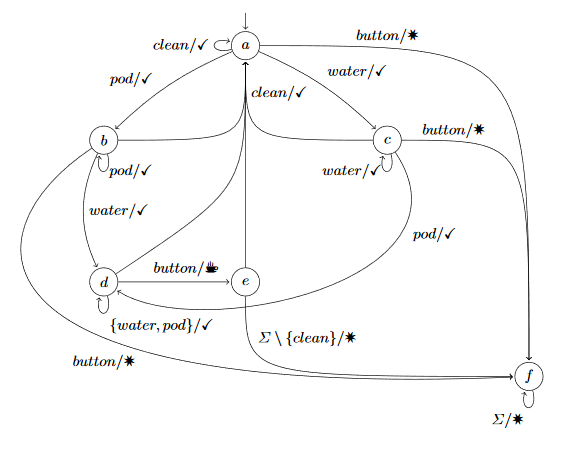
\includegraphics[width=0.7\linewidth]{figures/coffeemealyminimal}
	\caption{Minimal version of the Mealy machine seen in \ref{fig:coffeemealy}}
	\label{fig:coffeemealyminimal}
\end{figure}

Constructing automata to be canonical, especially in the case of Mealy machines is important with regards to efficiency and is the backbone of automata learning. The next proposition comes straightforward from the previously presented characterization theorem.


\noindent \textbf{Proposition (Bounded reachability\cite{Steffen2011})}: Every state of a minimal Mealy machine with n states has an access sequence, i.e., a path from the initial state to the given state,  of  length  at  most n-1.  Every  transition  of the model can be covered by a sequence of length at most n from the initial state.

The process of constructing automata uses the concept of partition refinement. It works based on distinguishing suffixes, suffixes of words which mark, witness the difference between two access sequences. The following notion is introduced to formalize this.


\begin{definition}[k-distinguishability\cite{Steffen2011}]
	Two states, $s,s'\in S$ are k-distinguishable iff there is a word $w\in\Sigma^*$ of length k or shorter, for which $\lambda^*(s, w)\neq\lambda^*(s',w)$.
\end{definition} 

\begin{definition}[exact k-distinguishability]
	Two states, $s,s'\in S$ are exact k-distinguishable, denoted by $k^=$ iff s and s' are k-distinguishable, but not (k-1)-distinguishable.
\end{definition}

Essentially, if two states, s and s' are  k-distinguishable, then when processing the same input sequence, from some suffix of the word w with length at most k, they will produce differing outputs. Using this, we can observe, that whenever two states, $s_1, s_2\in S$ are (k+1)-distinguishable, then they each have a successor $s_1'$ and $s_2'$ reached by some $\alpha\in\Sigma$, such that $s_1'$ and $s_2'$ are k-distinguishable. These successors are called $\alpha$-successors. This suggests, that:
\begin{itemize}
	\item no states are 0-distinguishable and
	\item two states $s_1$ and s2 are (k+1)-distinguishable iff there exists an input symbol $\alpha\in\Sigma$, such that $\lambda(s_1, \alpha) \neq \lambda(s_2,\alpha)$ or $\delta(s_1, \alpha)$ and $\delta(s_2, \alpha)$ are k-distinguishable.\cite{Steffen2011}
\end{itemize}
This way, if we have an automaton M, we can construct its minimal version, by iteratively computing k-distinguishability for increasing k, until stability, that is until the set of exactly k-distinguishable states is empty.

\begin{example}
	Given the Mealy machine seen in Figure \ref{fig:coffeemealy}, we can use k-distinguishability to refine its partitions. The initial state, the initial partition would be:\\
	$P_1 = \{a, b, c\}, \{d, d'\}, \{e\}, \{f\}$\\
	since when k=1, a, b and c are not 1-distinguishable, but d and d' separate on the behavior of the \textit{button} input, while e and f are separated by the suffix \textit{clean}. Let's see the k=2 scenario.\\
	$P_2 = \{a\}, \{b\}, \{c\}, \{d, d'\}, \{e\}, \{f\}$\\
	Here, \textit{water} and \textit{pod} separate a, b and c, while d and d' can still no longer be separated. If observed, even if k is increased, d and d' can not be refined. This means, that they are indistinguishable, they can be merged together without altering behavior. This shows the process of acquiring the minimal machine seen in Figure \ref{fig:coffeemealyminimal}.
	\label{ex:partitionrefinement}
\end{example} 

The process explained in Example \ref{ex:partitionrefinement} is partition refinement, the exact algorithm and proof of its validity can be seen in \cite{Steffen2011}. Partition refinement is a version of the minimization algorithm for DFAs proposed by Hopcroft\cite{HOPCROFT1971189}. 

Let us define one last relation which will be useful in the next section to compare automata minimization and automata learning.

\begin{definition}[k-epimorphisms]
	Let $M=(S,s_{0},\Sigma,\Omega,\delta,\lambda)$ and $M'=(S',s_{0}',\Sigma,\Omega,\delta',\lambda')$ be two Mealy machines with shared alphabets. We call a surjective function $f_k: S \to S'$ existential k-epimorphism between $M$ and $M'$, if for all $s'\in S', s\in S$ where $f_k(s) = s'$ and with any $\alpha\in\Sigma$, we have: $f_k(\delta(s,\alpha)) = \delta'(s',\alpha)$, and all states, that are mapped by $f_k$ to the same state of $M'$ are not k-distinguishable.
\end{definition}

It is straightforward to establish that all intermediate models arising during the partition refinement process are images of the considered Mealy machine under a k-epimorphism, where k is the number of times all transitions have been investigated.\cite{Steffen2011} Essentially this establishes $P_1$ and $P_2$ from Example \ref*{ex:partitionrefinement} as images of the Mealy machine seen in Figure \ref{ex:coffeemealy} under k-epimorphisms where k=1 and k=2 respectively. 

Active automata learning algorithms operate in a similar way, but they do not have access to the automata they are learning.

Note, that although it is possible -- and often quite useful -- to define minimal  $\omega$-automata (the one having the least number of states), however, several problems arise during the minimization process, due to not having a theorem resembling Theorem \ref{theorem:Myhill-Nerode} in this case. Firstly, there is no "canonical" acceptance condition: an automaton of one acceptance condition can have exponentially more states than another one with a different acceptance condition (both accepting the same language). In addition, there may be several, topologically different minimal automata with the same acceptance condition accepting the same language. This results in an NP-complete problem out of the scope of this thesis, thus, not discussed futher. For this reason, active automata learning algorithms for finite automata are not applicable for $\omega$-languages. 

\section{Automata Learning}

\paragraph{Automata Learning}  is a way of modeling a system without having specific knowledge of its internal behavior. To accomplish this, the external behavior of the system needs to be observed. This learned model is, as the name suggests, an automaton. 
\\Formally: Automata  learning is  concerned  with  the  problem  of  inferring  an automaton model for an unknown formal language $L$ over some alphabet $\Sigma$\cite{Howar2018}.
\\\\In order to monitor a system, access to its behavioral information is required. There are two approaches, which distinguish the two types of automata learning.

\paragraph{Passive Automata Learning} In case of passive automata learning, the gathering of information is not part of the learning process, but rather a prerequisite to it. The learning is performed on a pre-gathered positive an/or negative example set of the systems behavior. In passive automata learning, the success of the process is determined not only by the efficiency of the algorithm, but the methodology and time used to gather the data.

\paragraph{Active Automata Learning} In case of active automata learning, the behavioral information is gathered by the learning algorithm via queries. In order to accomplish this, learning is separated to two components: the learner, which learns, and the teacher, which can answer questions about the system under learning.


Active automata learning follows the MAT, or the Minimally Adequate Teacher model proposed by Dana Angluin\cite{ANGLUIN198787}. It defines the separation of the algorithm to a teacher and a learner component in a way, where the teacher can only answer the minimally adequate questions needed to learn the system. These two questions, or queries are are follows:


\paragraph{Membership query} Given a $w\in\Sigma^{*}$ word, the query return the $o\in \Omega$ output o corresponding to it, treating the word as a string of inputs. We write $mq(w) = o$ to denote that executing the query w on the system under learning (SUL) leads to the output o: $\llbracket SUL \rrbracket(w) = o$ or $\lambda^*(s_0, w) = o$.

\paragraph{Equivalence query} Given a hypothesis automaton $M$, the query attempts to determine if the hypothesis is behaviorally equivalent to the SUL, and if not, finding the diverging behavior, and return with an example. We write $eq(H) = c$, where $c\in\Sigma^*$, to denote an equivalence query on hypothesis H, returning a counterexample c. The counter example provided is the sequence of inputs for which the output of system under learning and the output of the hypothesis differ: $ \llbracket H\rrbracket(c) \neq mq(c)$.

\noindent The learner component uses membership queries to construct a hypothesis automaton, then refines this hypothesis by the counterexamples provided by equivalence queries. Once counterexamples can not be found this way, the learners hypothesis is behaviorally equivalent to the SUL. The learning can terminate and the output of the learning is the current hypothesis.

%TODO: diagram legyen korrekt uml
\begin{figure}[!ht]
	\centering
	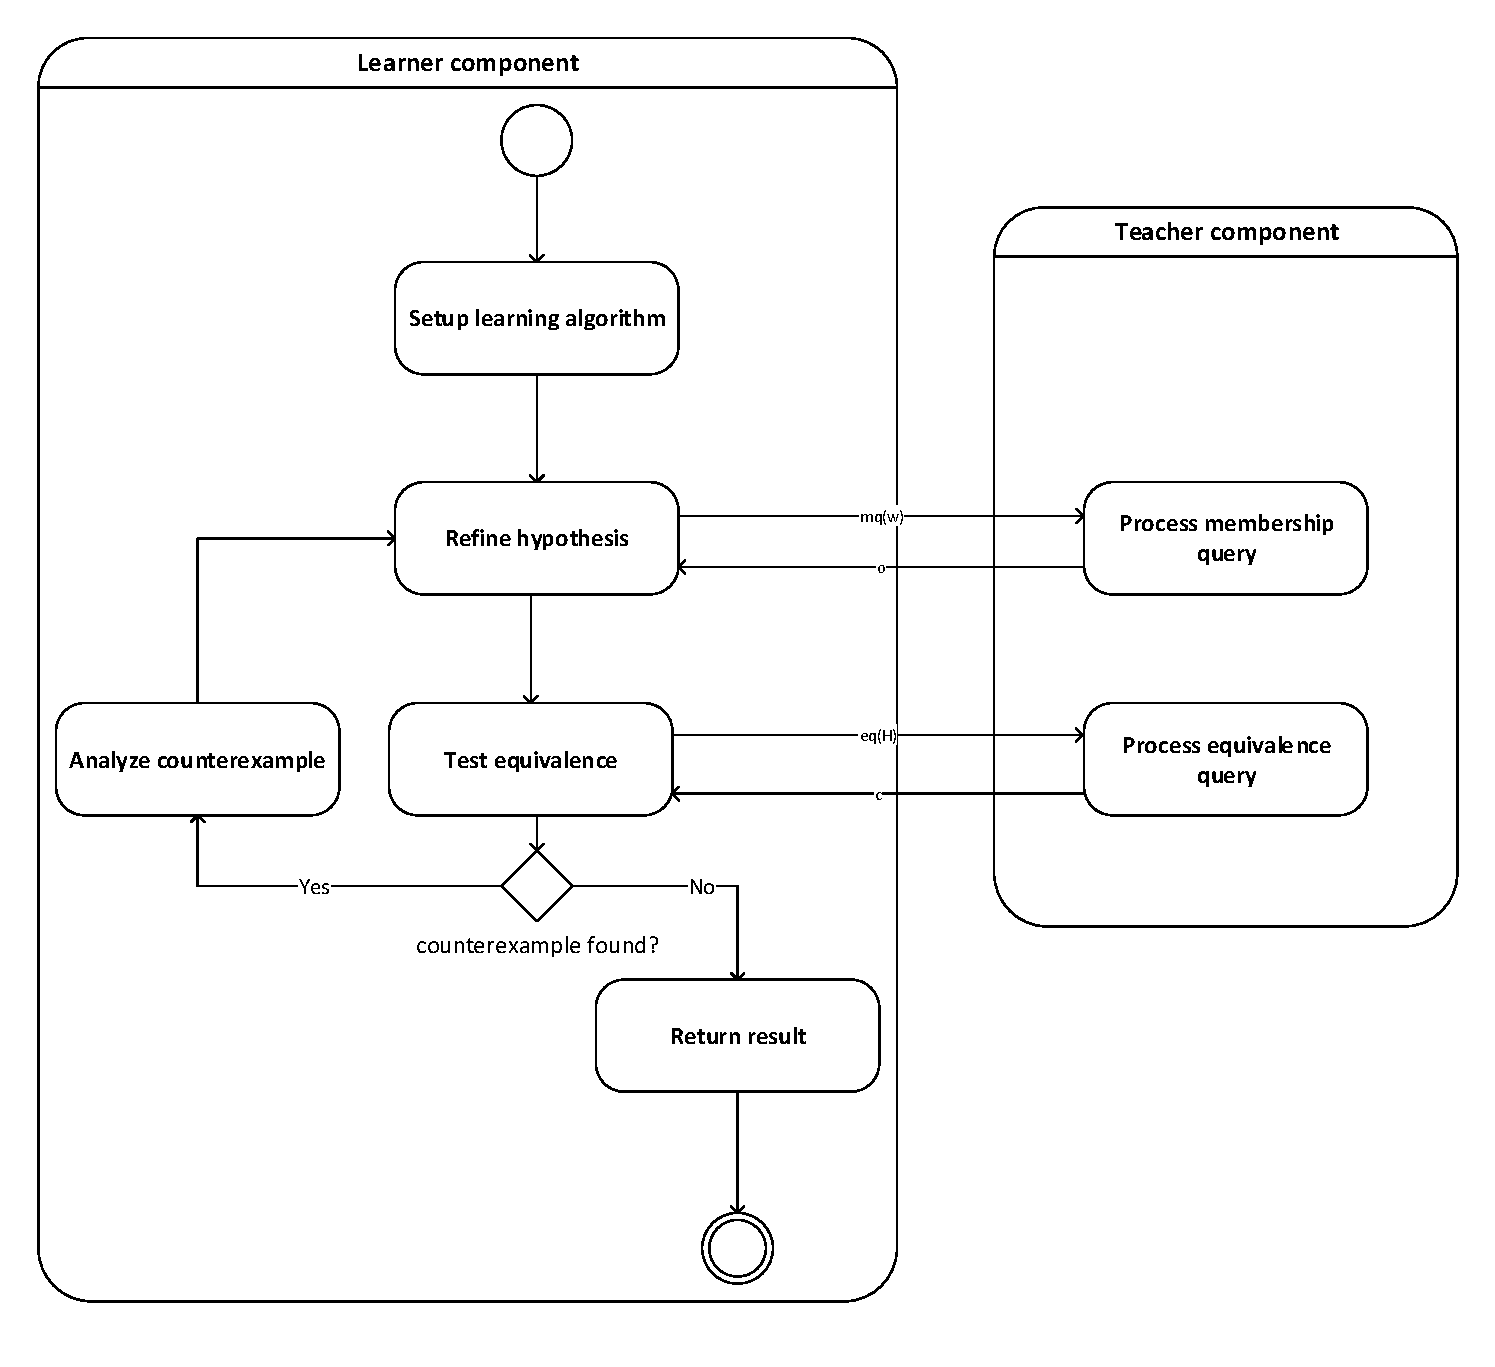
\includegraphics[width=1.0\linewidth]{figures/flowchartlearning}
	\caption{Active automata learning}
	\label{fig:flowchartlearning}
\end{figure}

As seen on Figure \ref{fig:flowchartlearning}, the learning proceeds in rounds, generating and refining hypothesis models by exploring the SUL via membership queries. As the equivalence checks produce counterexamples, the next round of this hypothesis refinement is driven by the counterexamples produced.

Using an analogous strategy to the minimization of automata seen in the previous section, starting only with a one state hypothesis automaton, all words are explored in the alphabet in order to refine and extend this hypothesis. Here, there is a dual way of characterizing (and distinguishing) between states\cite{Steffen2011}:
\begin{itemize}
	\item By words reaching them. A prefix-closed set $S_p$ of words, reaching each state exactly once, defines a spanning tree of the automaton. This characterization aims at providing exactly one representative element from each class of $\equiv_P$ on the SUL. Active learning algorithms incrementally construct such a set $S_p$. \\This prefix-closedness is necessary for $S_p$ to be a "spanning tree" of the Mealy machine. Extending $S_p$ with all the one-letter continuations of words in $S_p$ will result in the tree covering all the transitions of the Mealy machine. $L_p$ will denote all the one-letter continuations that are not already contained in $S_p$.
	\item By their future behavior with respect to an increasing vector of words of $\Sigma^*$. This vector $<d_1, d_2,...,d_k>$ will be denoted by $D$, and contains the "distinguishing suffixes". The corresponding future behavior of a state, here given in terms of its access sequence $u\in S_p$, is the output vector$<mq(u*d_1), ..., mq(u*d_k)>\in\Omega^k$, which leads to an upper approximation of the classes of $\equiv_{\llbracket SUL\rrbracket}$. Active learning incrementally refines this approximation by extending the vector until the approximation is precise.
\end{itemize}
While the second characterization defines the states of the automaton, where each output vector corresponds to one state, the spanning tree on $L_p$ is used to determine the transitions of these states. In order to characterize the relation between the SUL $M=(S,s_{0},\Sigma,\Omega,\delta,\lambda)$ and the hypothesis model $M'=(S',s_{0}',\Sigma,\Omega,\delta',\lambda')$ (note, that $M$ and $M'$ only share alphabets), the following definition is introduced. 

\begin{definition}[D-epimorphism]
	Let $D\subseteq\Sigma^*$. We call a surjective function $f_D:S\to S'$ existential D-epimorphism (surjective homomorphism) between $M$ and $M'$ if, for all $s'\in S'$ there exists an $s\in S$ with $f_D(s) = s'$ such that for all $\alpha \in \Sigma$ and all $d\in D$: $f_D(\delta(s, \alpha)) = \delta'(s', \alpha)$, and $\lambda^*(s,d) = \lambda^*(s', d)$. 
\end{definition}

Note, that active learning deals with canonical Mealy machines, in other words, the canonical form of SUL, and not, the perhaps much larger Mealy machine of SUL itself. 

Since active learning algorithms maintain an incrementally growing extended spanning tree for $H=(S_H, h_0, \Sigma, \Omega, \delta_H, \lambda_H)$, i.e., a prefix-closed set of words reaching all its states and covering all transitions, it is straightforward to establish that these hypothesis models are images of the canonical version of SUL under a canonical existential D-epimorphism, where D is the set of distinctive futures underlying the hypothesis construction\cite{Steffen2011}
\begin{itemize}
	\item define $f_D : S_{SUL}\to S_H$ by $f_D(s) = h$ as following: if $\exists w\in S_p \cup L_p$, where $\delta(s_0, w) = s$, then $h = \delta_H(h_0,w)$. Otherwise h may be chosen arbitrarily.
	\item It suffices to consider the states reached by words in the spanning tree to establish the defining properties of $f_D$. This straightforwardly yields:
	\begin{itemize}
		\item $f_D(\delta(s,\alpha)) = \delta_H(h, \alpha)$ for all $\alpha\in\Sigma$, which reflects the characterization from below.
		\item $\lambda^*(s, d) = \lambda^*_H(h,d)$ for all $d\in D$, which follows from the maintained characterization from above.\cite{Steffen2011}
	\end{itemize}
\end{itemize}

In basic logic, D-epimorphisms and k-epimorphisms do not differ, they both deal with establishing constructed models being images of the model they are based on. D-epimorphisms could replace k-epimorphisms where $D=\Sigma^k$, it can be suggested, that there is no need to differentiate. However, there is in important difference of complexity between the two. While k-distinguishability supports polynomial time, black-box systems do not. Also, the "existential" in existential D-epimorphism is important: $f_D$ must deal with unknown states, ones that haven't been encountered yet. This implies that characterization can only be valid for already encountered states.

Active learning algorithms can be proven correct using the following three-step pattern:
\begin{itemize}
	\item Invariance: The number of states of each hypothesis has an upper bound of $\equiv_{\llbracket SUL\rrbracket}$.
	\item Progress: Before the final partition is reached, an equivalence query will provide a counterexample, where an input word leads to a different output on the SUL and on the hypothesis. This difference can only be resolved by splitting at least one state, which increases the state count.
	\item Termination: The refinement terminates after at most the index of $\equiv_{\llbracket SUL\rrbracket}$ many steps, caused directly by the described invariance and progress properties.
\end{itemize}

The following subsection introduces basic active automata learning algorithms this thesis builds on.

\subsection{Basic Automata Learning Algorithms}
\textbf{Direct Hypothesis Construction (DHC):} 
The Direct Hypothesis Construction algorithm, which hypothesis construction can be seen in Algorithm \ref{algo:dhc}  follows the idea of the breath-first search of graph theory. It constructs the hypothesis using a queue of states, which is initialized with the states of the spanning tree to be maintained. Explored states are removed from this queue, while the discovered successors are enqueued, if they are provably new states. The algorithm starts with a one-state hypothesis, including only the initial state, reached by $\epsilon$ and D = $\Sigma$. It then tries to complete the hypothesis: for every state, the algorithm determines the behavior of the state under D. This behavior is called the extended signature of said state. States with a new extended signatures are provably new states, so to guarantee further investigation, all their successors are enqueued. Initially, $D=\Sigma$, so only the $1^=$-distinguishable states are revealed during the first iteration. This is extended straightforwardly to comprise a prefix closed set of access sequences. \cite{Steffen2011}\cite{10.1007/978-3-642-34781-8_19}

\begin{algorithm}[H]
	\SetAlgoLined
	\DontPrintSemicolon
	\KwIn{$S_p$: a set of access sequences, D: a set of suffixes, an input alphabet $\Sigma$}
	\KwOut{A Mealy machine $H=(S, s_0, \Sigma, \Omega, \delta, \lambda)$}
	initialize hypothesis H, create a state for all elements of $S_p$\;
	initialize a queue Q with the states of H\;
	\While{Q is not empty}{
		s = dequeue state from Q\;
		u = access sequence from $s_0$ to s\;
		\For{$d\in D$}{
			o = mq($u\*d$)\;
			set $\lambda(s,d) = o$\;
		}
		\eIf{exists an $s'\in S$, where the output signature of $s'$ is the same as $s$}{
			reroute transitions of $s$ to $s'$ in H\;
			remove $s$ from H\;
		}{
			create and enqueue successors of $s$ for every input in $\Sigma$ into Q, if not already in $S_p$\;
		}
	}
	Remove entries of $D\setminus\Sigma$ from $\lambda$\;
	\Return{H}\;
	\caption{Hypothesis construction of the Direct Hypothesis Construction algorithm as seen in \cite{Steffen2011}.}
	\label{algo:dhc}
\end{algorithm}

After the execution of the Hypothesis construction seen in Algorithm \ref{algo:dhc}, the output automaton H is used in an equivalence query $eq(H) = c$, to find if a counterexample $c$ exists. If no counteraxamle can be found, the learning terminates, $H$ is the learned automaton. Else, if a counterexample $c$ is found, for which $\lambda_H(s_0,c) \neq mq(c)$, $c$ is used to enlarge the suffixes in D and a new iteration of Algorithm \ref{algo:dhc} begins, using the now extended set D and all the access sequences found in the previous iteration (the current spanning tree $S_p$).

The DHC algorithm is a straightforward implementation of active automata learning. It terminates after at most $n^3mk+n^2k^2$ membership queries, and $n$ equivalence queries, where $n$ is the number of states in the final hypothesis, $k$ is the longest set of inputs, and $m$ is the length of the longest counterexample\cite{10.1007/978-3-642-34781-8_19}.



\boldmath{$L^*_M$} \textbf{Algorithm:}
\unboldmath
%TODO cite!!!
The $L^*_M$ algorithm -- seen in Algorithm \ref{algo:lstar} -- is similar to the DHC algorithm, however, it maintains a global table containing the previously gathered information. Informally, the rows of the table correspond to states and state candidates of the hypothesis, and are labeled with a possible access sequence of the given state (candidate). The columns of the table correspond to the suffixes of the access sequence containing separating behavior. Thus, the fields of the table are the results of $mq(prefix + suffix)$. The fields are indexed with $Obs(prefix, suffix)$.

More precisely, the rows are divided into two disjoint sets: $S_p$ contains unique rows, which correspond to the states during the hypothesis construction. $L_p$ contains rows, which are labeled with the labels of $S_p$ + an element from the input alphabet -- i.e. the continuation of the access sequences of $S_p$.

Before each hypothesis construction, the consistency and closedness of the table must be ensured. This means, that $S_p$ must only contain unique rows, and each row in $L_p$ must have a corresponding row in $S_p$ with the same elements. This can be reached by iteratively adding unique rows of $L_p$ to $S_p$ and adding their continuations to $L_p$. 

This algorithm results in a canonical automaton of the learned system, but does not ensure, that the intermediate hypotheses are minimal. That property requires $D$ to be semantically suffix-closed before the equivalence queries. We say that $D$ is semantically suffix-closed for the hypothesis $H$, if for any two states $u, u' \in S_p$ and any decomposition $v_1 v_2 \in D$ of any suffix with $Obs(u, v_1 v_2) \neq Obs(u', v_1 v_2)$. It is possible to ensure this property using a simple algorithm described together with the original one.

\begin{algorithm}[H]
	\SetAlgoLined
	\DontPrintSemicolon
	\KwIn{$\Sigma$: an input alphabet}
	\KwOut{A Mealy machine $H=(S, s_0, \Sigma, \Omega, \delta, \lambda)$}
	initialize table T (...) \\
	\While{true}{
		construct $H$ by algorithm Close Table \\
		\While{Check Semantic Suffix-Closedness returns a separator $d$}{
			$D := D \cup \{ d \}$ \\
			construct H by algorithm Close Table \\
		}
		counterExample := eq($H$) \\
		\If{counterExample is empty} {
			return $H$
		}
		$d$ := Process CounterExample \\
		$D := D \cup \{ d \}$
	}
	\Return{H}\;
	\caption{Hypothesis construction of the $L^*_M$ algorithm as seen in TODO CITE.}
	\label{algo:lstar}
\end{algorithm}

The $L^*_M$ algorithm is more refined implementation of automata learning than the DHC algorithm. Let $n$ denote the number of states in the final hypothesis and $k$ the size of the input alphabet. The algorithm terminates after at most $n^2k + k^2n + nlog(m)$ membership queries, the first two terms resulting from the maximum size of the table and the last term as a result of processing the equivalence queries. It also asks at most $n$ equivalence queries. Also, all computation that is required on the table and the construction of hypothesis models is polynomial in the size of the final observation table, which contains maximum $n^2k + k^2n$ elements.

\subsection{Advanced Approaches}
%TODO placeholder (better ones, variants, etc)
TODO

\section{Specifying Complex Requirements}
The previous sections introduced different modeling types and techniques. We now discuss the requirements used in model-based engineering which the models need to satisfy.

\subsection{Requirements and Properties}
Throughout this thesis, the concept of requirements is used widely, therefore, it is essential to define it precisely. 

\begin{definition}[Requirement\cite{sweterminology}]
	\mbox{}
	\begin{enumerate}
		\setlength\itemsep{0.1em}
		\item A condition or capability needed by the user to solve a problem or achieve an objective.
		\item A condition or capability that must be met or possessed by a system component to satisfy a contract, standard, specification or other formally imposed documents.
		\item A documented representation of a condition or capability as in (1) or (2).
	\end{enumerate}
\end{definition}

Basically, requirements are properties of the system, which the system must satisfy. They can be specified in many different ways, the most common being textual requirements in traditional feature lists. This method is an informal way of requirements specification, as the structure of this format is hard to analyze due to it lacking a precise definition. Attempts were made to formalize this type of requirements by defining patterns and mapping the individual patterns to formal semantics, however, there are also more abstract approaches, such as \textit{temporal logics}.

The rationale behind the precise formalization is the wide range of automated applications, especially in \textit{formal methods} -- such as validation, formal verification, test oracle generation and requirement documentation generation. The rest of this subsection defines basic concepts concerning properties.

\begin{definition}[Linear-Time Property]
	\label{def:ltproperty}
	A linear-time property (LT property) $P$ over the set of atomic propositions $AP$ is defined as $P \subseteq (2^{AP})^\omega$
	
	An LT property is thus an $\omega$-language over the alphabet $2^{AP}$.
\end{definition}

LT properties can be used to describe restictions on the traces of transition systems, such as LTSs (introduced in Subsection \ref{ss:automata}) or Kripke-structures \cite{Kripke1963-KRISCO}.

\begin{definition}[Satisfaction of LT Properties]
	\label{def:ltsatisfaction}
	Let $TS = (S, Act, \rightarrow)$ be a (labeled) transition system, $AP = Act$ the set of atomic propositions and $P$ an LT property over $AP$. $TS$ satisfies $P$ -- denoted $TS \vDash P$ -- iff $Traces(TS) \subseteq P$.
	
	This means, that a transition system $TS$ satisfies the LT property $P$, if all its traces respect $P$.
\end{definition}

\begin{example}
	\label{ex:ltpropexample}
	Figure \ref{fig:ltpropexample} depicts a system of two fully synchronized traffic lights, each only having two possible actions: red and green. The set of atomic propositions is $AP = \{red_1, green_1, red_2, green_2\}$.
	
	Consider the LT property: $P=$ "The first traffic light is infinitely often green." This corresponds to the set of infinite words of the form $A_0A_1A_2...$, such that $green_1 \in A_i$ holds for infinitely many $i$. \\\\
	Examples of such infinite words include:
	\begin{itemize}
		\item {$\{green_1\}\emptyset\{green_1\}\emptyset\{green_1\}\emptyset\{green_1\}\emptyset$$\dots$}
		\item {$\{red_1,green_2\}\{green_1,red_2\}\{red_1,green_2\}\{green_1,red_2\}$$\dots$}
	\end{itemize}
	Examples of infinite words not included in $P$:
	\begin{itemize}
		\item {$\{red_1,green_1\}\{red_1,green_1\}\emptyset\emptyset\emptyset$$\dots$ -- it contains finitely many occurrences of $green_1$}
		\item {$\{red_1,red_2\}\{red_1,red_2\}\{red_1,red_2\}$$\dots$ -- it contains no occurrences of $green_1$}
	\end{itemize}

	Naturally, finite words do not satisfy $P$ -- by definition, they never satisfy LT properties.

	It is easy to see, that both the model of the first controller (Figure \ref{fig:trafficLTS_1}) and the product controller (Figure \ref{fig:trafficLTS_3}) satisfy $P$.
\end{example}

\begin{figure}[!ht]
	\centering
	\begin{subfigure}[b]{0.2\textwidth}
		\centering
		\begin{tikzpicture}[shorten >=1pt,node distance=3cm,on grid,auto] 
			\node[state, initial] (q_0)   {$q0$}; 
			\node[state] (q_1) [below=of q_0] {$q1$}; 
			
			\path[->] 
			(q_0) edge [bend left=25] node {$red_1$} (q_1)
			(q_1) edge [bend left=25] node {$green_1$} (q_0);
		\end{tikzpicture}
		\caption{1st controller}
		\label{fig:trafficLTS_1}
	\end{subfigure}
	\hfill
	\begin{subfigure}[b]{0.2\textwidth}
		\centering
		\begin{tikzpicture}[shorten >=1pt,node distance=3cm,on grid,auto] 
			\node[state, initial] (q_2) [right=5cm of q_0] {$q0$}; 
			\node[state](q_3) [below=of q_2] {$q1$};
			
			\path[->] 
			(q_2) edge [bend left=25] node {$green_2$} (q_3)
			(q_3) edge [bend left=25] node {$red_2$} (q_2);
		\end{tikzpicture}
		\caption{2nd controller}
		\label{fig:trafficLTS_2}
	\end{subfigure}
	\hfill
	\begin{subfigure}[b]{0.5\textwidth}
		\centering
		\begin{tikzpicture}[shorten >=1pt,node distance=3cm,on grid,auto] 
			\node[state, initial] (q_0)   {$ \langle q0,q0 \rangle $}; 
			\node[state] (q_1) [below=of q_0] {$ \langle q1,q1 \rangle $}; 
			
			\path[->] 
			(q_0) edge [bend left=45] node {$red_1$,$green_2$} (q_1)
			(q_1) edge [bend left=45] node {$green_1$,$red_2$} (q_0);
		\end{tikzpicture}
		\caption{Product automaton}
		\label{fig:trafficLTS_3}
	\end{subfigure}
	
	\caption{A simplified model of two fully synchronized traffic lights based on \cite{principlesofmodelchecking}}
	\label{fig:ltpropexample}
\end{figure}

Following the natural distinction between what a modeled system \textit{should} and what it \textit{should not} do, it is possible to introduce the terms \textit{safety} and \textit{liveness} properties.

\begin{definition}[Safety Property]
	An LT property $P_{safe}$ over $AP$ is called a \textit{safety} property iff for all words $\sigma \in (2^{AP})^\omega \backslash P_{safe}$ there exists a finite prefix $\hat{\sigma}$ of $\sigma$ such that $P_{safe} \cap \{\sigma' \in \sigma \in (2^{AP})^\omega | \hat{\sigma}$ is a finite prefix of $\sigma'\} = \emptyset$.
	
	In that case, $\hat{\sigma}$ is called a \textit{bad prefix}. A \textit{minimal bad prefix} is a bad prefix of minimal length.
\end{definition}

\begin{definition}[Liveness Property]
	An LT property $P_{live}$ over $AP$ is called a \textit{liveness} property iff for all finite words $w \in (2^{AP})^*$ there exists an infinite word $\sigma \in (2^{AP})^\omega$ satisfying $w \sigma \in P$.
\end{definition}

\begin{theorem} 
	The only LT property over $AP$ that is both a safety and a liveness property is $(2^{AP})^\omega$. \cite{principlesofmodelchecking}
\end{theorem}

\begin{theorem}
	For any LT property $P$ over $AP$, there exists a safety property $P_{safe}$ and a liveness property $P_{live}$ such that $P = P_{safe} \cap P_{live}$. \cite{principlesofmodelchecking}
\end{theorem}

\begin{example}
	\label{ex:safetyliveness}
	Consider the property "the machine provides tea infinitely often after initially providing coffee three times in a row" regarding a vending machine. This can be decomposed into two parts.
	
	The first part -- "provides tea infinitely often" -- is a liveness property: any finite trace can be extendid such that the property holds.
	
	The second part -- "initially providing coffee three times in a row" -- is a safety property: any finite trace in which one of the first three drinks is tea (or generally, not coffee) violates it.
\end{example}


There is also a third aspect frequently mentioned in the literature: \textit{fairness} properties. These are assumptions that rule out infinite behaviors that are considered unrealistic, and are often necessary to establish liveness properties. However, they are out of the scope of this thesis and are not detailed further.

The class of $\omega$-lanugages resulting from the above definition of LT properties is too general to handle. For simpler (i.e. decidable) processing and verification of these properties, we restrict the language of the properties to $\omega$-regular languages. We will see, that this is enough in most practical use-cases.

\begin{definition}[$\omega$-Regular Properties]
	\label{def:omegaregprop}
	An LT property $P$ over the set of atomic propositions $AP$ is called $\omega$-regular, if $P$ is an $\omega$-regular language over the alphabet $2^{AP}$.
\end{definition}

More complex constructs also exist in the literature, but these raise serious problems -- such as undecidability -- like context-free extensions introduced in \cite{temporallogics}. 
	
In the following subsection, we are going to introduce languages for the specification of different LT properties.


\subsection{Linear-Time Temporal Logic}
Linear-Time Temporal Logic (LTL), also called Propositional Linear-Time Temporal Logic (PLTL) is the extension of propositional logic with temporal connectives over \textit{paths} of a \textit{base model}, e.g. an LTS. It is common to use definitions using Kripke-structures \cite{Kripke1963-KRISCO} as base models too, depending on the application. The syntax of LTL expressions over paths of LTSs is defined as follows:

\begin{definition}[Syntax of LTL Expressions]
	Let $\pi = (s_0, a_1, s_1, a_2, ... )$ be a path of an LTS. Then the valid LTL expressions can be derived using the following production rules:
	\begin{itemize}
		\item $L_1$: if $a \in Act$, then $(a)$ is an LTL expression. 
		\item $L_2$: if $p$ and $q$ are LTL expressions, then $p \land q$ and $\neg p$ are LTL expressions.
		\item $L_3$: if $p$ and $q$ are LTL expressions, then $p U q$ and $X p$ are LTL expressions.
	\end{itemize}
	With the operator precedence: $\leftrightarrow$  <<  $\rightarrow$  << $\land$  <<  $\neg$  <<  $X, U$
\end{definition}

Additional operators can also be defined using the already defined ones:
\begin{itemize}
	\setlength\itemsep{0.2em}
	\item $true$ holds for every state,
	\item $false$ does not hold for any state,  
	\item $p \lor q$ as $\neg((\neg p) \land (\neg q))$,
	\item $p \rightarrow q$ as $(\neg p) \lor q$,
	\item $p \leftrightarrow q$ as $(p \rightarrow q) \land (q \rightarrow p)$,
	\item $F p$ as $true U p$,
	\item $G p$ as $\neg F(\neg p)$,
	\item $p WB q$ as $\neg((\neg p) U q)$,
	\item $p B q$ as $\neg((\neg p) U q) \land F q$
\end{itemize}

The semantics of LTL expressions are defined as follows:
\begin{definition}[Semantics of LTL Expressions]
	\label{def:ltlsemantics}
	Let $\pi = (s_0, a_1, s_1, a_2, ... )$ be a trace of an LTS model $M=(S, Act, \rightarrow)$. Then the formal semantics to the LTL expressions $a$, $p$ and $q$ is given recursively, with regard to syntactic production rules as:
	\begin{itemize}
		\item $L_1$: $M,\pi \vDash (a) \leftrightarrow a_1 = a$ 
		\item $L_2$: $M,\pi \vDash p \land q$ $\leftrightarrow$  $M,\pi \vDash p$ and  $M,\pi \vDash q$; \\
		$M,\pi \vDash \neg q$ $\leftrightarrow$ not  $M,\pi \vDash q$
		\item $L_3$: $M,\pi \vDash (p U q)$ $\leftrightarrow$  $\exists j \geq 0$ : $\pi^j \vDash q$ and $\forall 0 \leq k \leq j : \pi^k \vDash p$; \\
		$M,\pi \vDash X p$ $\leftrightarrow$ $\pi^1 \vDash p$
	\end{itemize}
	Where $\vDash$ is the logical entailment operator, $M,\pi \vDash q$ denoting: for trace $\pi$ of model $M$, $q$ holds.
	
\end{definition}

\begin{example}
	\label{ex:ltlexample}
	Based on these definitions, Figure \ref{fig:ltlexample} shows examples for the intuitive meanings of different LTL operators.
\end{example}

\begin{figure}[!ht]
	\centering
	\begin{subfigure}[b]{0.9\textwidth}
		\centering
		\begin{tikzpicture}[shorten >=1pt,node distance=2cm,on grid,auto] 
			\node[state] (s_1)   {}; 
			\node[state] (s_2) [right=of s_1] {}; 
			\node[state] (s_3) [right=of s_2] {}; 
			\node[state](s_4) [right=of s_3] {};
			\node[state](s_5) [right=of s_4] {};
			\path[->] 
			(s_1) edge  node {} (s_2)
			(s_2) edge  node {} (s_3)
			(s_3) edge  node {p} (s_4)
			(s_4) edge  node {} (s_5);
		\end{tikzpicture}
		\caption{$F p$}
	\end{subfigure}
	\hfill
	\begin{subfigure}[b]{0.9\textwidth}
		\centering
		\begin{tikzpicture}[shorten >=1pt,node distance=2cm,on grid,auto] 
			\node[state] (s_1)   {}; 
			\node[state] (s_2) [right=of s_1] {}; 
			\node[state] (s_3) [right=of s_2] {}; 
			\node[state](s_4) [right=of s_3] {};
			\node[state](s_5) [right=of s_4] {};
			\path[->] 
			(s_1) edge  node {p} (s_2)
			(s_2) edge  node {p} (s_3)
			(s_3) edge  node {p} (s_4)
			(s_4) edge  node {p} (s_5);
		\end{tikzpicture}
		\caption{$G p$}
	\end{subfigure}
	\hfill
	\begin{subfigure}[b]{0.9\textwidth}
		\centering
		\begin{tikzpicture}[shorten >=1pt,node distance=2cm,on grid,auto] 
			\node[state] (s_1)   {}; 
			\node[state] (s_2) [right=of s_1] {}; 
			\node[state] (s_3) [right=of s_2] {}; 
			\node[state](s_4) [right=of s_3] {};
			\node[state](s_5) [right=of s_4] {};
			\path[->] 
			(s_1) edge  node {} (s_2)
			(s_2) edge  node {p} (s_3)
			(s_3) edge  node {} (s_4)
			(s_4) edge  node {} (s_5);
		\end{tikzpicture}
		\caption{$X p$}
	\end{subfigure}
	\begin{subfigure}[b]{0.9\textwidth}
		\centering
		\begin{tikzpicture}[shorten >=1pt,node distance=2cm,on grid,auto] 
			\node[state] (s_1)   {}; 
			\node[state] (s_2) [right=of s_1] {}; 
			\node[state] (s_3) [right=of s_2] {}; 
			\node[state](s_4) [right=of s_3] {};
			\node[state](s_5) [right=of s_4] {};
			\path[->] 
			(s_1) edge  node {p} (s_2)
			(s_2) edge  node {p} (s_3)
			(s_3) edge  node {q} (s_4)
			(s_4) edge  node {} (s_5);
		\end{tikzpicture}
		\caption{$p U q$}
	\end{subfigure}
	
	\caption{Intuitive examples for the meanings of different LTL operators}
	\label{fig:ltlexample}
\end{figure}

LTL expressions over paths of LTS models can be used to formulate requirements for any system interpretable as LTSs (such as Mealy machines) in a formalized way resembling conventional propositional logic -- which is widely used among engineers. LTL is a well-researched area of mathematics, and has an extensive tooling available for different purposes. One such application is the transformation to $\omega$-automata, which then can be executed parallel with the modeled system to verify its behavior.

\begin{example}
	\label{ex:ltlbuchi}
	Figure \ref{fig:ltlToBuchi} shows a possible transition-based Generalized Büchi Automaton corresponding the LTL specification $(GFa) \leftrightarrow (GFb)$. A run is accepting if it visits both edges marked with \textcolor{orange}{0} and \textcolor{cyan}{1} infinitely often.
\end{example}

\begin{figure}[!ht]
	\centering
	\begin{tikzpicture}[shorten >=1pt,node distance=3cm,on grid,auto] 
		\node[state, initial] (q_0)   {$0$}; 
		\node[state] (q_1) [above right=of q_0] {$1$}; 
		\node[state] (q_2) [below right=of q_0] {$2$};
		
		\path[->] 
		(q_0) edge [loop above] node {$\top$} (q_0)
		(q_0) edge node [below right] {$\neg a \neg b$} (q_1)
		(q_1) edge [loop right] node [below right] {$\neg a \neg b$} node [above right] {\{\textcolor{orange}{0}, \textcolor{cyan}{1}\}} (q_1)
		(q_0) edge node [left] {$a \lor b$} (q_2)
		(q_2) edge [loop above] node [above left] {$a b$} node [above right] {\{\textcolor{orange}{0}, \textcolor{cyan}{1}\}} (q_2)
		(q_2) edge [loop right] node [below right] {$a \neg b$} node [above right] {\{\textcolor{orange}{0}\}} (q_2)
		(q_2) edge [loop below] node {$\neg a \neg b$} (q_2)
		(q_2) edge [loop left] node [below left] {$\neg a b$} node [above left] {\{\textcolor{cyan}{1}\}} (q_2);
	\end{tikzpicture}
	\caption{A transition-based GBA for the specification $(GFa) \leftrightarrow (GFb)$}
	\label{fig:ltlToBuchi}
\end{figure}

Based on Definition \ref{def:ltlsemantics}, it can be shown that LTL expressions are only capable of describing $\omega$-regular LT properties. On the other hand, LTL only possesses the expressive power to describe a proper subset of all $\omega$-regular languages \cite{firstorderdefinable}. This makes room for extensions and different property specification approaches, which are discussed in the following subsections.

\subsection{Extensions of LTL}

TODO

\section{Reactive Synthesis from Temporal Logic}

The previous section defined requirements and properties. A straightforward way of utilizing these requirements in connection with automata learning is to transform them to its targeted formalism -- a Mealy automaton. Luckily, model synthesis from $\omega$-regular LT properties is a well-researched area with an extensive literature. In this section, we are going to introduce the most common synthesis techniques from such properties to Mealy automata. 

%TODO insert reference(s) to definition(s)
From the definition of $\omega$-regular properties follows, that an $\omega$-automaton must exist for each $\omega$-regular property. We have also seen, that several formalisms exist for the formulation of $\omega$-regular properties, each fit for a different subset of these properties. Thus, we are only going to discuss the problem of finding an appropriate controller -- in this case a Mealy machine -- for a given $\omega$-automaton.  

\subsection{Synthesis Problem for Reactive Systems}
Formally, an instance of the \textit{reactive synthesis problem} is a triple $(I,O,L)$, where $I$ and $O$ are two disjoint sets of input and output events (words) respectively, and $L$ is an $\omega$-regular language over the alphabet $2^{I \cup O}$ -- given as an $\omega$-automaton. 

A \textit{controller} is a function $C : (2^{I \cup O})^* \times 2^I \rightarrowtail 2^O$. An infinite word $u = u_0 u_1 u_2 \dots \in (2^{I \cup O})^\omega$ is \textit{consistent} with controller C if, for every $n \in \mathbb{N}, u_n \cap O = C(u_0, \dots, u_n \cap I)$. A controller $C$ is said to \textit{enforce} $L$ if every infinite word consistent with $C$ is in $L$. Given $I$, $O$ and $L$, the reactive synthesis problem asks, whether there exists a controller enforcing $L$, and asks for a witness if the answer is positive. \cite{ltlsynt}

From this triple-based definition of the reactive synthesis problem, game theory and the formal definition of games is a natural association.

\subsection{Games and Reactive Systems}

A \textit{game} is an $\omega$-automaton, where the set of states $Q$ is partitioned into two sets $Q_A$ and $Q_B$ for two players $A$ and $B$. We refer to the underlying automaton (seen as an automaton and not as a game) as its \textit{arena}. Runs of the arena are called \textit{plays} in the game setting. By convention, the acceptance condition of the arena is the winning condition for the second player ($B$) in the game: a play is won by B if and only if it is accepting in the arena. Otherwise, the play is won by A (in particular, finite plays are won by A). It is also convenient to partition $\Sigma$ into $\Sigma_A$ (letters played by A) and $\Sigma_B$ (letters played by B). This restricts $\Delta$ (the transition relation) of the $\omega$-automaton so that transitions from $Q_A$ and $Q_B$ are labelled with letters from $\Sigma_A$ and  $\Sigma_B$ respectively.

A \textit{strategy} for A (resp. B) is a function mapping finite plays ending in $Q_A$ (resp. $Q_B$) to a valid transition extending the play. Given a strategy $\sigma$ for A (resp. B), a $\sigma$-play is a (finite or infinite) play $\rho$ where every transition taken by A (resp. B), say at position i, is given by $\sigma ( \rho_0 \dots \rho_i)$. A \textit{positional} (or \textit{memoryless}) strategy is a strategy whose value depends only on the state in which the given run ends. Given one strategy for each player, say $\sigma_A$ and $\sigma_B$, there is a unique longest play that is both a $\sigma_A$-play and a $\sigma_B$-play, which is called the outcome of $\sigma_A$ and $\sigma_B$. A winning strategy for a player is a strategy that makes that player win its outcome against every strategy for the other player. A game is \textit{turn-based} if $\Delta$ alternates between $Q_A$ and $Q_B$ (i.e. no player plays twice in a row).

It is now clear, that the thus defined games and the reactive synthesis problem are closely related -- just swap the players A and B to the I and O of the synthesis problem -- and the old and well-researched game-theory can be applied to efficiently solve it.

In fact, most state-of-the-art approaches -- such as LTLSYNT \cite{ltlsynt} and STRIX \cite{strix} -- use parity-game solving for model synthesis, which we discuss next.
%\subsection{Bounded Synthesis through Safety Games}

\subsection{Synthesis through Parity Games}

The $\omega$-automata, based on which the controller is constructed, does not necessarily separate input and output symbols. This results in smaller automata -- perfect for verification -- that are hard to utilize in model synthesis. Thus, we need to define a corresponding intermediate formalism, which takes this into consideration.

\begin{definition} [Split Word, Language, Automaton]
Let a \textit{word} $u = (u_i)_{i \in \mathbb{N}} \in (2^{I \cup O})^\omega$. We define $split_{I,O}(u) = (v_i)_{i \in \mathbb{N}} \in (2^I 2^O)^\omega$ as follows: for all $i \in \mathbb{N}$, $v_{2i} = u_i \cap I$ and $v_{2i+1} = ui \cap O$. This operation naturally extends to \textit{languages}: $split_{I,O}(L) = \{split_{I,O}(u) | u \in L \}$.

The split of an \textit{automaton} $A = (Q,2^{I \cup O}, \Delta, q_0, F)$ is the automaton, noted $split_{I,O}(A)$, $(Q \cup Q \times 2^I, 2^{I \cup O},\Delta_s,q_0,F)$ where each transition $(q,a,f,q_0) \in \Delta$ gives, for each $i \in a \cap 2^I$, two transitions in $\Delta_s$: $(q,i,\emptyset,(q,i))$ and $((q,i),a \cap 2^O,f,q')$.
\end{definition}

\begin{example}
	\label{ex:splitexample}
	Figure \ref{fig:splitexample} shows an example of a split automaton for the Büchi-automaton of Example \ref{ex:ltlbuchi}. Notice, how the splitting separates the edges to ones containing only input symbols and those containing only output symbols. Also note, that the split automaton is nondeterministic and exhibits the acceptance condition of the original automaton: the transition-based generalized Büchi condition.
\end{example}

\begin{figure}[!ht]
	\centering
	\begin{tikzpicture}[shorten >=1pt,node distance=3cm,on grid,auto] 
		\node[state, initial] (q_0)   {$0$}; 
		\node[state] (q_1) [above=of q_0] {$3,\neg a$};
		\node[state] (q_11) [right=of q_1] {$2$};
		\node[state] (q_12) [above right=of q_11] {$2,\neg a$};
		\node[state] (q_13) [below right=of q_11] {$2, a$};   
		\node[state] (q_2) [below=of q_0] {$3, a$};
		\node[state] (q_21) [right=of q_2] {$1$};
		\node[state] (q_22) [above right=of q_21] {$1, \neg a$};
		\node[state] (q_23) [below right=of q_21] {$1, a$};
		
		\path[->] 
		(q_0) edge [bend left=40] node [left] {$\neg a$} (q_1)
		(q_1) edge [bend left=40] node [left] {$\top$} (q_0)
		(q_1) edge node {$\neg b$} (q_11)
		(q_11) edge [bend left=40] node {$\neg a$} (q_12)
		(q_12) edge [bend left=40] node [above right, circle, fill=white, draw=cyan, thick] {\small \textcolor{cyan}{\textbf{1}}} node [below left, circle, fill=white, draw=orange, thick] {\small \textcolor{orange}{\textbf{0}}} node [right=0.5] {$\neg b$} (q_11)
		(q_11) edge node [left] {$a$} (q_13)
		(q_0) edge [bend left=40] node [left] {$a$} (q_2)
		(q_2) edge [bend left=40] node [left] {$\top$} (q_0)
		(q_2) edge node {$\top$} (q_21)
		(q_21) edge [bend left=40] node [above] {$\neg a$} (q_22)
		(q_22) edge node [left] {$\neg b$} (q_21)
		(q_22) edge [bend left=40] node [below left=-0.5, circle, fill=white, draw=cyan, thick] {\small \textcolor{cyan}{\textbf{1}}} node [right=0.4] {$b$} (q_21)
		(q_21) edge [bend left=40] node [right] {$a$} (q_23)
		(q_23) edge [bend left=40] node [below right=-0.1, circle, fill=white, draw=orange, thick] {\small \textcolor{orange}{\textbf{0}}} node [above left=0.1, circle, fill=white, draw=cyan, thick] {\small \textcolor{cyan}{\textbf{1}}} node [below left=0.1] {$b$} (q_21)
		(q_23) edge node [below left=-0.35, circle, fill=white, draw=orange, thick] {\small \textcolor{orange}{\textbf{0}}} node [above=0.2] {$\neg b$} (q_21)
		(q_1) edge [bend left=20] node {$b$} (q_21);
	\end{tikzpicture}

	\caption{Split automaton of the automaton from Figure \ref{fig:ltlToBuchi} based on \cite{ltlsynt}.}
	\label{fig:splitexample}
\end{figure}

For the construction of an appropriate controller, the following two theorems give clues. For the proofs, we refer the reader to \cite{ltlsynt}.

\begin{theorem}
	Let $G$ be a game whose arena is complete and deterministic for player $A$ and that recognizes $split_{I,O}(L)$. If player $B$ wins $G$, then there is a controller enforcing $L$.
\end{theorem}
\begin{theorem}
	Let $G$ be a game whose arena is complete for $A$, deterministic (for both players) and recognizes the language $split_{I,O}(L)$. If there is a controller enforcing $L$, then $B$ wins the game $G$.
\end{theorem}

Note, that both theorems require the arena of the game to be deterministic, and no algorithms are known for the nondeterministic case. This restricts the applicability of certain $\omega$-automata, as, e.g. deterministic Büchi-automata are strictly less expressive than their nondeterministic counterparts. Thus, most approaches use deterministic parity automata (DPA) as the arena of the games to solve. Deterministic and nondeterministic parity automata are equally able to express all $\omega$-regular languages and they also have a natural association to turn-based games. Thus, the next step of these synthesis algorithms is the determinization of the input $\omega$-automata by applying a transformation to a DPA. A possible algorithm for the transformation of transition-based Büchi-automata to transition-based DPA is that of Redziejowski \cite{redziejowski}.

This is followed by the solution of the parity game. An appropriate algorithm is Zielonka's recursive algorithm \cite{zielonka}, with the time complexity of $O(n^d)$, where $d$ is the number of different priorities in the game. There are other, quasi-polinomial algorithms too, which can be applied with little improvement in most practical cases.

\begin{example}
	\label{ex:paritygameexample}
	Figure \ref{fig:paritygameexample} shows a parity game constructed from the automaton in Example \ref{ex:splitexample} -- with a deterministic parity automaton as its arena. The diamond nodes belong to Player A -- the environment player -- and the circular nodes belong to player B -- the system player. Player B wins, if the minimum priority encountered infinitely often is odd. 
	
	The solution is also shown: the highlighted nodes and transitions are in the winning strategy, while the grey elements are unreachable.
\end{example}

\begin{figure}[!ht]
	\centering
	\begin{tikzpicture}[shorten >=1pt,node distance=1.5cm,on grid,auto] 
		% INITIAL
		\node[diamond, draw, initial] (q_0)   {$$}; 
		% RIGHT OF THE INITIAL
		\node[circle, draw] (q_11) [above right=of q_0] {$$};
		\node[diamond, draw, gray] (q_12) [right=of q_0]   {$$}; 
		\node[circle, draw] (q_13) [below right=of q_0] {$$};
		\node[circle, draw, gray] (q_14) [right=of q_12] {$$};
		% FIRST BOTTLENECK 
		\node[diamond, draw] (q_2) [right=of q_14]   {$$};
		% RIGHT OF THE FIRST BOTTLENECK
		\node[circle, draw] (q_31) [above right=of q_2] {$$};
		\node[diamond, draw] (q_32) [right=of q_2]   {$$};
		\node[circle, draw] (q_33) [below right=of q_2] {$$};
		\node[circle, draw] (q_34) [right=of q_32] {$$};
		% SECOND BOTTLENECK
		\node[diamond, draw, gray] (q_4) [right=of q_34]   {$$};
		% RIGHT OF THE SECOND BOTTLENECK
		\node[circle, draw, gray] (q_51) [right=of q_4] {$$};
		\node[diamond, draw, gray] (q_52) [above=of q_51]   {$$};
		\node[circle, draw, gray] (q_53) [right=of q_51] {$$};
		
		\path[->] 
		% FIRST BLOCK (INIT <-> FIRST BOTTLENECK)
		(q_0) edge [bend left=40] node [left] {$\neg a$} (q_11)
		(q_11) edge [gray] node [left] {$\neg b$} (q_12)
		(q_12) edge [gray] node [left] {$a$ $\{0\}$} (q_13)
		(q_0) edge [bend right=40] node [left] {$a$} (q_13)
		(q_12) edge [bend left=40, gray] node [above] {$\neg a$ $\{1\}$} (q_14)
		(q_14) edge [bend left=40, gray] node [below] {$\neg b$ $\{1\}$} (q_12)
		(q_14) edge [gray] node [below] {$b$ $\{0\}$} (q_2)
		(q_11) edge [bend left=40] node [above] {$b$} (q_2)
		(q_13) edge [bend right=40] node [below] {$\top$} (q_2)
		% SECOND BLOCK (FIRST <-> SECOND BOTTLENECK)
		(q_2) edge [bend left=40] node [above] {$a$} (q_31)
		(q_31) edge [gray] node [above] {$\neg b$} node [left=-0.3cm] {$\{2\}$} (q_2)
		(q_31) edge [bend left=40] node [below] {$b$$\{1\}$} (q_2)
		(q_2) edge [bend right=40] node [below] {$\neg a$} (q_33)
		(q_33) edge node [right] {$\neg b$} (q_32)
		(q_32) edge node [right=-0.4cm] {$a$ $\{2\}$} (q_31)
		(q_32) edge [bend left=40] node [above] {$\neg a$ $\{3\}$} (q_34)
		(q_34) edge [bend left=40] node [below] {$\neg b$ $\{3\}$} (q_32)
		(q_34) edge [gray] node [below] {$b$ $\{2\}$} (q_4)
		(q_4) edge [bend right=40, gray] node [above] {$a$ $\{1\}$} (q_31)
		(q_33) edge [bend right=40, gray] node [below] {$b$} (q_4)
		% THIRD BLOCK (SECOND -> ETC)
		(q_4) edge [bend left=40, gray] node [above] {$\neg a$} (q_51)
		(q_51) edge [bend left=40, gray] node [above] {$b$ $\{2\}$} (q_4)
		(q_51) edge [gray] node [left] {$\neg b$} (q_52)
		(q_52) edge [bend right=40, gray] node [above] {$a$ $\{1\}$} (q_31)
		(q_52) edge [bend left=40, gray] node [above] {$\neg a$ $\{3\}$} (q_53)
		(q_53) edge [bend left=40, gray] node [above] {$\neg b$ $\{3\}$} (q_52)
		(q_53) edge [bend left=40, gray] node [below] {$b$ $\{2\}$} (q_4)
		;
	\end{tikzpicture}
	
	\caption{Parity game from the automaton on Figure \ref{fig:splitexample} based on \cite{ltlsynt}.}
	\label{fig:paritygameexample}
\end{figure}

When Player B has a winning strategy $\sigma$ from the initial state, we can extract a controller from $\sigma$ that ensures realisation of the specification. It corresponds to an incompletely specified Mealy machine, where some outputs might not be specified and could be instantiated either way. This enables more compact representations and retains the possiblities in the implementations.

Let $(V_A , V_B, E)$ be the parity game arena where B wins from the initial state with the strategy $\sigma$. We can use $Q = \{q \in V_A |$ Player B wins the game applying the strategy $\sigma\}$ as the set of states. For the transition function, let $\delta(q, i) := q′$ by choosing some $q′$ where $((q, I), O, q') \in \sigma$ for some $I \subseteq \Sigma_{in}$ with $i \in I$ and any $O \subseteq \Sigma_{out}$. By construction, and as $\sigma$ is a winning strategy for all $q \in Q$, such a $q′$ always exists. However, there may be multiple applicable $q′$. This may result in several possible -- not necessarily minimal -- controllers. For the output function, let $\delta(q,i) = q'$ be an edge of the Mealy machine. Then, let $\lambda(q,i) = \{o$ | $\exists I,O : i \in I$ and $o \in O$ and $((q,I),O,q) \in \sigma\}$ -- a Boolean formula encoding all the possible corresponding outputs in a nondeterministic way.

\begin{example}
	Figure \ref{fig:synthmealyexample} shows a Mealy automaton constructed from the winning strategy of the parity game in Example \ref{ex:paritygameexample}.
	
	Note, that the automaton is nondeterministic -- not fully specified -- and non-minimal -- $q_1$ and $q_2$ could be merged.
\end{example}

\begin{figure}[!ht]
	\centering
	\begin{tikzpicture}[shorten >=1pt,node distance=3cm,on grid,auto] 
		\node[state, initial] (0)  {$q_0$}; 
		\node[state] (1) [right of=0] {$q_1$}; 
		\node[state] (2) [right of=1] {$q_2$}; 
				
		\path[->] 
		(0) edge [bend left=40] node [above] {$\neg a / b$} (1)
		(0) edge [bend right=40] node [below] {$a / \Sigma_{out}$} (1)
		(1) edge [loop above] node [above] {$a / b$} (1)
		(1) edge [bend left=40] node [above] {$\neg a / \neg b$} (2)
		(2) edge [bend left=40] node [below] {$a / b$} (1)
		(2) edge [loop above] node [above] {$\neg a / \neg b$} (2)
		;
	\end{tikzpicture}
	
	\caption{Mealy machine from the parity game on Figure \ref{fig:paritygameexample}.}
	\label{fig:synthmealyexample}
\end{figure}

